\documentclass[xcolor=dvipsnames]{beamer}
\usepackage[czech]{babel}
\usepackage[utf8]{inputenc}
\usepackage{times}
\usepackage[T1]{fontenc}
\usepackage{lmodern}
\usepackage{graphicx}
\usepackage{url}
\usepackage{hyperref}
\usepackage{xmpmulti}
\usepackage{caption}
\usepackage{subcaption}


% Nastavení beameru:
\usetheme{Frankfurt}
\usecolortheme[named=blue]{structure}   	 	
\setbeamertemplate{items}[ball]                  % ball, circle, rectangle, default
\setbeamertemplate{blocks}[rounded][shadow=true] % zaobleni boxu a stiny
\setbeamertemplate{navigation symbols}{}         % vypne navigacni symboly

% uprava spodnich informacnich list
\setbeamertemplate{footline} {%
 % see beamer/themes/outer/beamerouterthemeinfolines.sty
  \leavevmode%
  \hbox{%
  \begin{beamercolorbox}[wd=.2\paperwidth,ht=2.25ex,dp=1ex,center]{author in head/foot}%
    \usebeamerfont{author in head/foot}\insertshortauthor %~~(\insertshortinstitute)
  \end{beamercolorbox}%
  \begin{beamercolorbox}[wd=.6\paperwidth,ht=2.25ex,dp=1ex,center]{title in head/foot}%
    \usebeamerfont{title in head/foot}\insertshorttitle{}
  \end{beamercolorbox}%
  \begin{beamercolorbox}[wd=.2\paperwidth,ht=2.25ex,dp=1ex,right]{date in head/foot}%
    \usebeamerfont{date in head/foot}\insertshortdate{}\hspace*{2ex}
    \insertframenumber{} / \inserttotalframenumber\hspace*{2ex}
  \end{beamercolorbox}}%
  \vskip0pt%
}

% Tohle rozchodi tecky v zahlavi prezentace:
\usepackage{remreset}
\makeatletter
\@removefromreset{subsection}{section}
\makeatother
\setcounter{subsection}{1}

%\def\itemtitle#1{{\usebeamercolor[fg]{item}\bfseries#1\smallskip}}
\def\itemtitle#1{{\bfseries#1\smallskip}}
\def\myverb#1{{\footnotesize\texttt{#1}\normalsize}}

% Informace o dokumentu pro titulni stránku a informacni listy
\subtitle{Obhajoba diplomovej práce}
\title[Ochrana elektronických dokumentov]{Ochrana elektronických dokumentov}
\author[Bc. Martin Bajaník]{Bc. Martin Bajaník}
\institute[FI MU]{Fakulta informatiky\\Masarykova univerzita\\\texttt{396204@mail.muni.cz}}
\date[10. 2. 2017]{Brno, 10. februára 2017}

% PDF settings
\hypersetup{%
unicode=true,                % čeština v záložkách
pdfpagelayout=SinglePage,    % SinglePage, OneColumn, TwoColumnLeft, TwoColumnRight
pdfstartview=FitV,           % Fit, FitB, FitH, FitV
pdftitle   = {Analyza sifrovanej prevadzky},
pdfauthor  = {Martin Bajanik - 396204@mail.muni.cz},
pdfsubject = {Fakulta informatiky, Masarykova univerzita},
pdfkeywords= {SSL, TLS, šifrovaná prevádzka, OpenSSL, FlowMon, IPFIX},
pdflang    = {cs}
}

% ----- The next line is important when dealing with alpha channels
% see http://bmeps.sourceforge.net/examples.html
\pdfpageattr {/Group << /S /Transparency /I true /CS /DeviceRGB>>}

\begin{document}

%------------------------------- titulní slide -------------------------------%

\section{Úvod}
\begin{frame}
  \titlepage
\end{frame}


%-----------------------------------------------------------------------------%

\begin{frame}
	\frametitle{Cieľ diplomovej práce}	
	\begin{itemize}
		\item Poskytnúť ucelený prehľad ochrán, implementovaných v najrozšírenejších formátoch, s dôrazom na ochranu dôvernosti dokumentov založenej na heslách. 
		\item Vytvoriť distribuovaný systém na obnovu zabudnutého hesla.
		\item Pomocou vytvoreného nástroja zhodnotiť schopnosť formátov odolať útokom hrubou silou a použitelnosť systému na obnovu hesla.  
	\end{itemize}
	
\end{frame}

%----------------------------------- Úvod ------------------------------------%

\section{Ochrana elektronických dokumentov}
\begin{frame}\frametitle{Ochrana elektronických dokumentov}
	\itemtitle{Spôsob ochrany}
	\begin{itemize}
		\item Šifrovanie - dôvernosť
		\item Digitálne podpisy - autenticita a integrita
	\end{itemize}
	\bigskip
	\itemtitle{Populárne formáty}
	\begin{figure}[h]
		\centering
		\includegraphics[width=100mm]{images/docs_logos.pdf} \\
		\vspace{-1mm}		
	\end{figure}
\end{frame}

%----------------------------------- Úvod ------------------------------------%

\begin{frame}\frametitle{Šifrovanie na základe hesla}
	\begin{figure}[h]
		\centering
		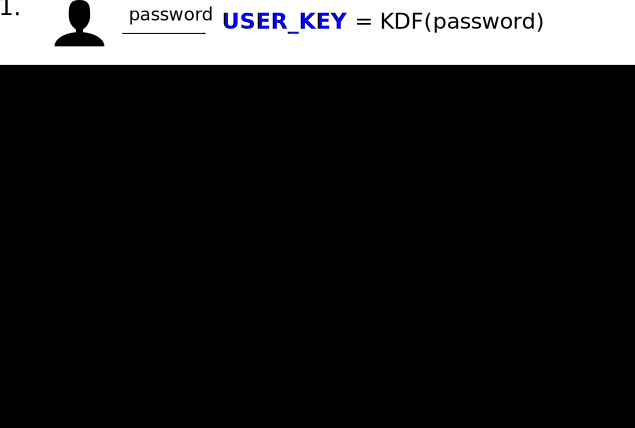
\includegraphics[width=100mm]{images/password_encryption_schema.pdf} \\
		\vspace{-1mm}		
	\end{figure}
\end{frame}

%-----------------------------------------------------------------------------%

\begin{frame}
	\frametitle{MS Office Document Cryptography Structure}
	\itemtitle{Šifrovanie na základe hesla}
	\begin{itemize}
		\item Open Office XML (ECMA-376)
		\item Štandardné šifrovanie (Office 2007)
		\begin{itemize}
			\item 50 000 iterácií
			\item SHA-1
		\end{itemize}
		\item Agilné šifrovanie (Office 2010 a vyššie)
		\begin{itemize}
			\item 100 000 iterácií
			\item SHA-1
			\item Konfigurovateľné užívateľom
		\end{itemize}
	\end{itemize}
\end{frame}

%-----------------------------------------------------------------------------%


\begin{frame}
	\frametitle{Portable Document Format}
	\itemtitle{Šifrovanie na základe hesla}
	\begin{itemize}
		\item Samostatný šifrovací modul (\textit{Standard Security Handler}) 
		\item PDF 1.1 - 1.3
		\begin{itemize}
			\item 50 iterácií MD5
		\end{itemize}
		\item PDF 1.4 - 1.7
		\begin{itemize}
			\item 50 iterácií MD5 a 19 iterácií RC4
		\end{itemize}
		\item PDF 1.7 s modulom verzie 5
		\begin{itemize}
			\item 1 iterácia SHA-256
		\end{itemize}
		\item PDF 1.7 s modulom verzie 6
		\begin{itemize}
			\item 32 iterácií SHA-2 a AES-128
		\end{itemize}
	\end{itemize}	
\end{frame}

%-----------------------------------------------------------------------------%

\begin{frame}
	\frametitle{Open Document Format}
	\itemtitle{Šifrovanie na základe hesla}
	\begin{itemize}
		\item Verzia 1.0 - 1.2
		\begin{itemize}
			\item 1024 iterácií PBKDF2 s HMAC-SHA1 (RFC 2898)
			\item Počet iterácií konfigurovateľný
		\end{itemize}
	\end{itemize}
\end{frame}

%-----------------------------------------------------------------------------%

\section{Distribuovaný systém na obnovu hesla}
\begin{frame}
	\itemtitle{Kľučové vlastnosti}
	\begin{itemize}
		\item Klient -- server architektúra
		\item Modularita a paralelizmus
	\end{itemize}
	\bigskip
	\begin{figure}[h]
		\centering
		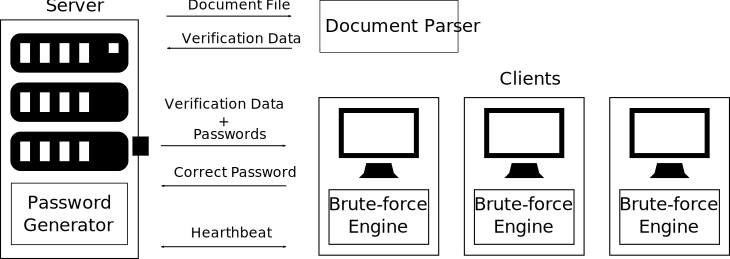
\includegraphics[width=100mm]{images/ddpbf_design.pdf} \\	
		\bigskip
		\scriptsize{Návrh systému na obnovu zabudnutého hesla}	
	\end{figure}
\end{frame}

%-----------------------------------------------------------------------------%

\begin{frame}
	\frametitle{Obnova hesla dokumentov hrubou silou}
	
	\begin{figure}[h]
		\centering
		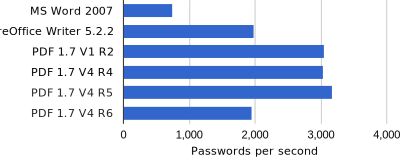
\includegraphics[width=100mm]{images/average_speed.pdf} \\	
		\bigskip
		\scriptsize{Priemerná rychlosť verifikácie správnosti hesla (počet pokusov za sekundu)}	
	\end{figure}
\end{frame}

%-----------------------------------------------------------------------------%

\section{Záver}
\begin{frame}
	\frametitle{Záver}

	\itemtitle{Hlavné prínosy práce}
	\begin{itemize}
		\item Ucelený popis ochrán implemetovaných v populárnych formátoch elektronických dokumentov.
		\item Zhodnotenie dostupných ochrán a testovanie odolnosti voči útokom hrubou silou. 
		\item Vytvorený funkčný distribuovaný systém na obnovu zabudnutého hesla s dôrazom na:
		\begin{itemize}
			\item rozšíriteľnosť vďaka modulárnemu prístupu,
			\item efektívnosť vďaka paralelizácii na viac úrovniach a
			\item jednoduchú použiteľnosť.
		\end{itemize}
	\end{itemize}
\end{frame}

%-----------------------------------------------------------------------------%

\begin{frame}
   \frametitle{Otázky}
 	\vspace*{\fill}

 	\begin{center} 		
 		\huge\bfseries\usebeamercolor[fg]{item} Ďakujem za pozornosť.\\~\\
 	\end{center}
 	\vspace*{\fill}
 \end{frame}

%-----------------------------------------------------------------------------%

\begin{frame}
	\frametitle{Otázky z posudkov}
	\begin{itemize}
		\item Co je to veřejná část certifikátu X.509?
		\item Zajímavé by bylo zmínit, proč byla vybrána MS právě tato fixní hesla (strana 11).
		\item Jsou násobné podpisy (např. v sekci 3.3:2) na stejné úrovni nebo hierarchicky řazené?
	\end{itemize}
\end{frame}

%-----------------------------------------------------------------------------%

\begin{frame}
	\frametitle{Štandardné vs. agilné šifrovanie}
	\begin{itemize}
		\item Binárny formát vs. XML
		\item Fixné algoritmy a parametre vs. CNG (\textit{CryptoAPI: Next Generation})
		\item Šifrovací kĺúč (tzv. \textit{intermediate key})
		\item Integrita (\textit{Encrypt then MAC}). 
	\end{itemize}
\end{frame}

%-----------------------------------------------------------------------------%

\begin{frame}
	\frametitle{Obnova hesla dokumentov hrubou silou}
	
	 \begin{table}[h]
	\centering
	\begin{tabular}{|l|l|l|l|}
           \hline
		&\textbf{MS Word 2007}&\textbf{LibreOffice Writer 5.2.2}&\textbf{PDF 1.7 V4 R5}\\
	\hline
		3&< 25 seconds&< 9 seconds&< 6 seconds\\
	\hline
		4&< 10 minutes&< 4 minutes&< 2.5 minutes\\
	\hline
		5&< 5 hours& < 2 hours&< 1.1 hours\\
	\hline
		6&< 5 days&< 2 days&< 1.2 days\\
	\hline
		7&< 17 weeks&< 7 weeks&< 4.2 weeks\\
	\hline
		8&< 9 years&< 3.5 years&< 2.1 years\\
	\hline
           \end{tabular}
	\end{table}
\begin{center}	
	\vspace{-5mm}
	\scriptsize{Odhadovaný čas na dokončenie procesu obnovy hesla danej dĺžky.}
\end{center}
\end{frame}

%-----------------------------------------------------------------------------%

\begin{frame}
\frametitle{Ďaľšie ochrany}
	\itemtitle{Ochrana proti zápisu (MS Office)}
	\begin{itemize}
		\item  Uplatnenie iba z pohľadu UX.
	\end{itemize}
	\bigskip
	\itemtitle{Šifrovanie pomocou asymetrickej kryptografie (PDF)}
	\begin{itemize}
		\item Dokument šifrovaný pomocou RC4.	
	\end{itemize}
	\bigskip
	\itemtitle{Digitalné podpisy}
	\begin{itemize}
	\item Microsoft Office a Open Document Format
	\begin{itemize}
		\item  XML Signature Syntax and Processing (W3C)
	\end{itemize}
	\item Portable Document Format
	\begin{itemize}
		\item  Pokročilá funkcionalita a robustné algoritmy.
	\end{itemize}
	\end{itemize}
\end{frame}

%-----------------------------------------------------------------------------%

\begin{frame}
\frametitle{Porovnanie implementácii ODT}
	\itemtitle{Apache OpenOffice vs. LibreOffice}
	\begin{table}[h]
	\centering
	\begin{tabular}{|l|l|l|}
               \hline
		&\textbf{LibreOffice}&\textbf{Apache OpenOffice}\\
	\hline
		checksum-type&SHA-256&SHA-1\\
	\hline
		algorithm-name&AES-256&Blowfish CFB\\
	\hline
		start-key-derivation-name&SHA-256&SHA-1\\
		key-derivation-name&PBKDF2&PBKDF2\\
		iteration-count&1024&1024\\
		key-size&32&16\\
	\hline
           \end{tabular}
	\end{table}
\end{frame}

%-----------------------------------------------------------------------------%

\begin{frame}
\frametitle{Šifrovanie dokumentov - algoritmy}
	\begin{itemize}
	\item Microsoft Office
	\begin{itemize}
		\item  Štandardné šifrovanie - AES-128, AES-192, AES-256 (ECB)
		\item Agilné šifrovanie - Windows OS API (CNG)
	\end{itemize}
	\item Portable Document Format
	\begin{itemize}
		\item RC4, AES-128 (CBC)
		\item Dĺžky kľúčov 40-128 bitov
	\end{itemize}
	\item Open Document Format
	\begin{itemize}
		\item  1.0 a 1.1 - Blowfish CFB
		\item 1.2 - Triple DES, AES-128, AES-192, AES-256 (CBC)
		\begin{itemize}
			\item XML Encryption Syntax and Processing (W3C)
		\end{itemize}
	\end{itemize}
	\end{itemize}
\end{frame}

\end{document}
